\newcommand{\econtexRoot}{Paper/}
% The \commands below are required to allow sharing of the same base code via Github between TeXLive on a local machine and ShareLaTeX.  This is an ugly solution to the requirement that custom LaTeX packages be accessible, and that ShareLaTeX seems to ignore symbolic links (even if they are relative links to valid locations)
\providecommand{\econtex}{\econtexRoot/texmf-local/tex/latex/econtex}
\providecommand{\econtexSetup}{\econtexRoot/texmf-local/tex/latex/econtexSetup}
\providecommand{\econtexShortcuts}{\econtexRoot/texmf-local/tex/latex/econtexShortcuts}
\providecommand{\econtexBibMake}{\econtexRoot/texmf-local/tex/latex/econtexBibMake}
\providecommand{\econtexBibStyle}{\econtexRoot/texmf-local/bibtex/bst/econtex}
\providecommand{\notes}{\econtexRoot/texmf-local/tex/latex/handout}
\providecommand{\handoutSetup}{\econtexRoot/texmf-local/tex/latex/handoutSetup}
\providecommand{\handoutShortcuts}{\econtexRoot/texmf-local/tex/latex/handoutShortcuts}
\providecommand{\handoutBibMake}{\econtexRoot/texmf-local/tex/latex/handoutBibMake}
\providecommand{\handoutBibStyle}{\econtexRoot/texmf-local/bibtex/bst/handout}

  

\documentclass{beamer}
\usepackage{remreset}
\usepackage{etoolbox}
\usepackage{comment}
\usepackage{graphicx}
%\usepackage{dtklogos}
\usepackage{dsfont}
\usepackage{amsmath,amssymb}
\usepackage{econtexShortcuts}
\usepackage[english]{babel}
\usepackage{tikz} 
\usepackage{cancel}
\usepackage{booktabs,natbib}
\setbeamercovered{invisible}

\usepackage{dcolumn}


\makeatletter
\@removefromreset{subsection}{section}
\patchcmd{\beamer@part}{\setcounter{subsection}{0}}{}{}
\makeatother
\setcounter{subsection}{1}
\setbeamercovered{transparent}

\mode<presentation>{}
%% preamble
\title[Income Uncertainty and Consumption Dynamics]{Income Uncertainty and Consumption Dynamics}
\author{Edmund Crawley \& Andreas Kuchler}
\date[6/21/2018]{June 21, 2018}
\usetheme{Frankfurt}
\begin{document}
\newcolumntype{d}[1]{D{.}{.}{#1}}
%circled draws a circle around a number
\newcommand*\circled[1]{\tikz[baseline=(char.base)]{
		\node[shape=circle,draw,inner sep=2pt] (char) {#1};}}


\frame{\titlepage}

\section{Motivation}
\setbeamercovered{invisible}
\frame
{
	\frametitle{Overview}
	What will this paper do?\\
	\begin{itemize}	
	\item[1] Create a new method to estimate heterogeneity in consumption responses to permanent and transitory shocks to income
	\item[2] Show how well a standard consumption saving model, calibrated to Danish data, fits
	\item[3] Application: Redistribution Channel of Monetary Policy (\cite{auclert_monetary_2015})
	\end{itemize}	
}
\frame{
	\frametitle{How Are Consumption Responses Typically Measured?}
	Three methods:
	\begin{itemize}
		\item[1] (Natural) Experiments - stimulus checks, lotteries etc
		\begin{itemize}
			\item Few true experiments, especially for permanent shocks
			\item Data limitations
		\end{itemize}
		\item[2] Ask people
		\begin{itemize}
			\item Unclear how to interpret
		\end{itemize}
		\item[3] Use covariance structure of income and consumption
		\begin{itemize}
			\item Empirical methods (until now!) have been flawed
		\end{itemize}
	\end{itemize}
	\pause
	Our contribution
	\begin{itemize}
		\item Develop a robust method based on 3
		\item Apply it to Danish registry data
\end{itemize}
The Danish data allows us to build a detailed picture of the distribution over different household characteristics
}
\frame
{
	\frametitle{Evidence on Magnitude of Consumption Response}
	\resizebox{\textwidth}{!}{
	\centering
		\input ../Tables/MPCLiterature.tex }
\tiny{$^{\star}$ Elasticity. Methods: 1) Natural Experiment 2) Survey question 3) Covariance restrictions} \\
\scriptsize Rough consensus on (3 month) transitory MPC $\sim 30\%$
}
\frame
{
	\frametitle{Evidence on Distribution of Consumption Response}
	Auclert (2018) uses the 3 different methods to identify the distribution of MPC by unhedged interest rate exposure
	\begin{figure}
		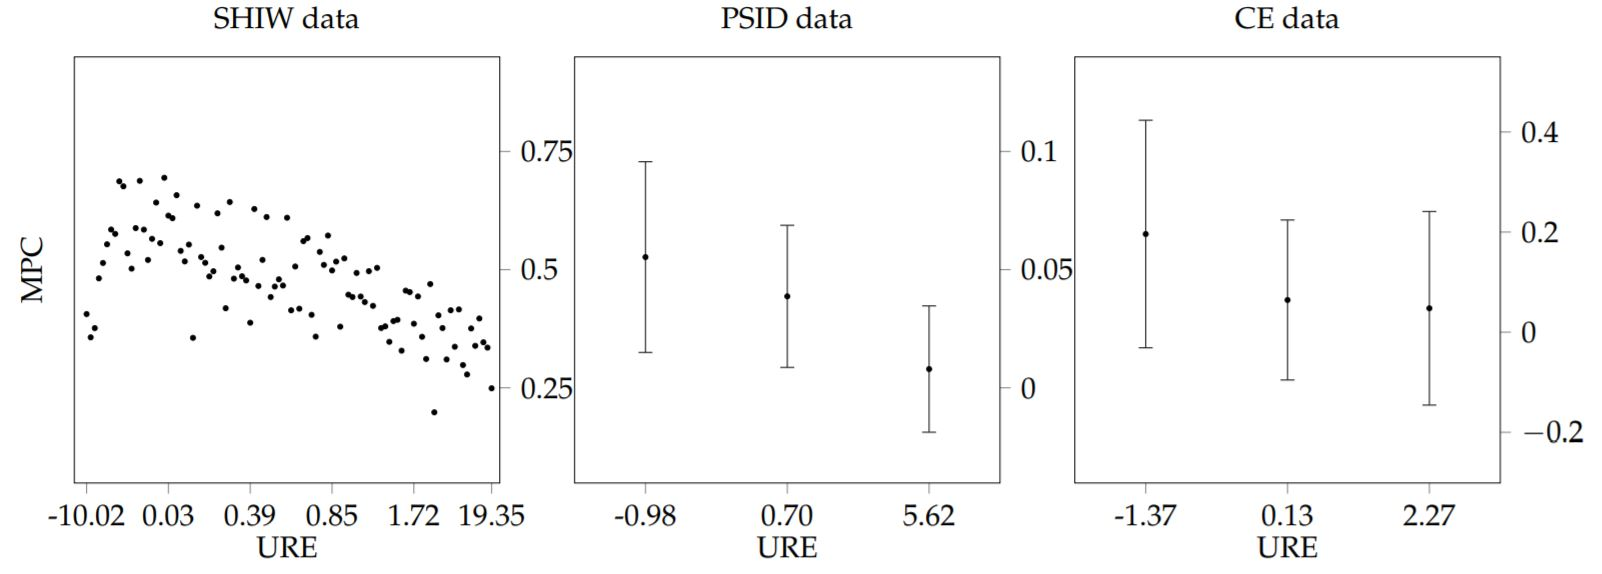
\includegraphics[scale=0.6]{../Figures/MPCDistributionAuclert}
	\end{figure}
	Recent evidence from Norwegian registry data using lottery winnings provides evidence of variation across liquid wealth
}
\frame{
	\frametitle{Results Preview}
	\begin{figure}
	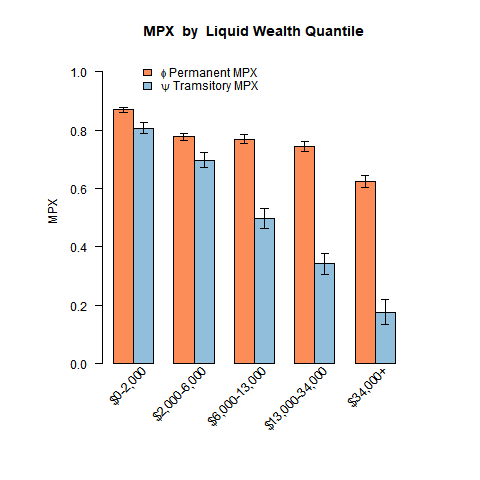
\includegraphics[scale=0.5]{../Figures/MPXByLiquidWealth_level_lincome_head.png}
	\end{figure}
}
\section{Empirical Strategy}
\setbeamercovered{invisible}
\frame
{
	\frametitle{Methodology Intuition}
	Exploit increasing importance of permanent shocks as the time over which growth is measured increases
	\begin{columns}
	\column{0.6\linewidth}
	\centering
	\begin{tikzpicture}
	\node (img1) {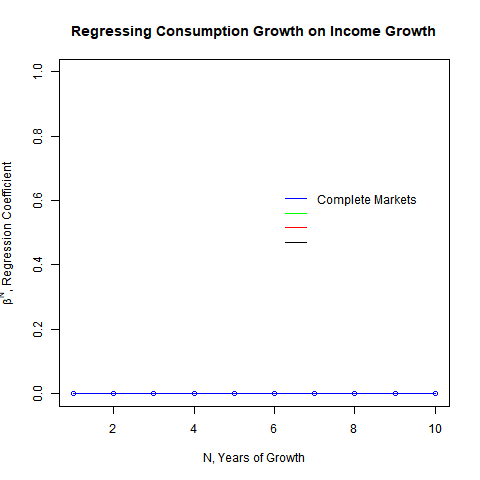
\includegraphics[height=6.5cm]{../Figures/basic_regression_complete_level_lincome_head.png}};
	\pause
	\node (img2) {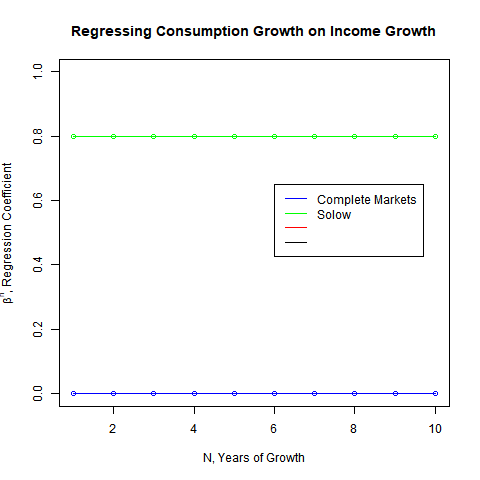
\includegraphics[height=6.5cm]{../Figures/basic_regression_solow_level_lincome_head.png}};
	\pause
	\node (img3) {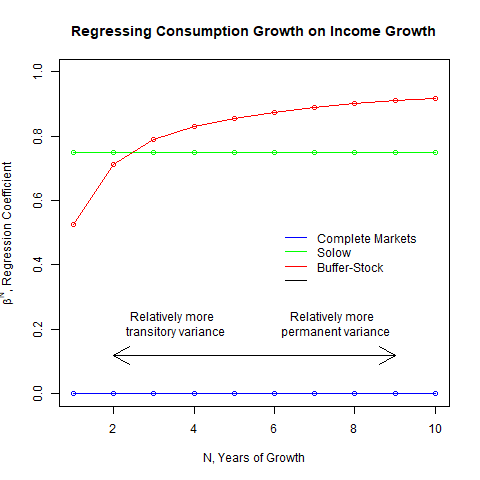
\includegraphics[height=6.5cm]{../Figures/basic_regression_BS_level_lincome_head.png}};
	\pause
	\node (img4) {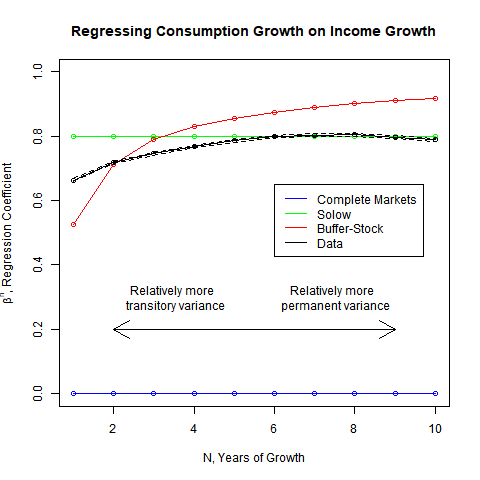
\includegraphics[height=6.5cm]{../Figures/basic_regression_level_lincome_head.png}};
	\pause
	\node (img5) {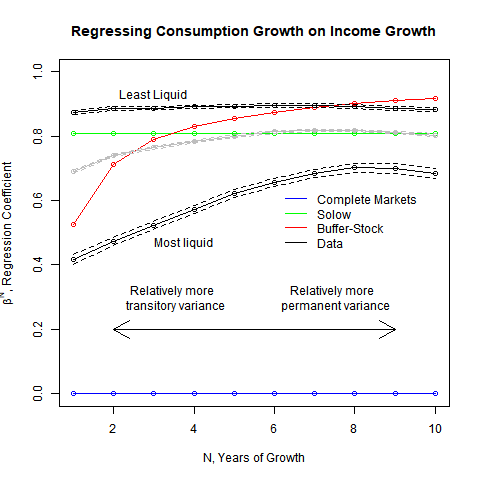
\includegraphics[height=6.5cm]{../Figures/basic_regression_liquid_wealth_level_lincome_head.png}};
	\end{tikzpicture}
	\column{0.4\linewidth}
	\begin{align*}
	\Delta^N c = \beta^N \Delta^N y +\varepsilon
	\end{align*}
	\end{columns}

}
\frame
{
	\frametitle{Aside: Why Not Blundell, Pistaferri and Preston 2008?}
	1) Time Aggregation Problem (Crawley 2018)
	\begin{columns}
	\column{0.5\linewidth}
	\centering
	\onslide<1->{
	\begin{tikzpicture}
	\node (img1) {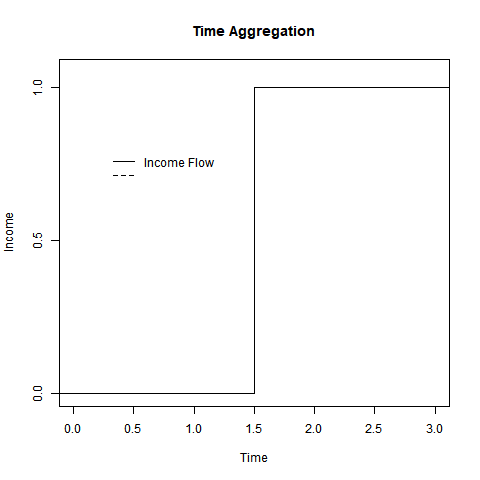
\includegraphics[height=5cm]{../Figures/TimeAggExample1.png}};
	\onslide<2->{
	\node (img2) {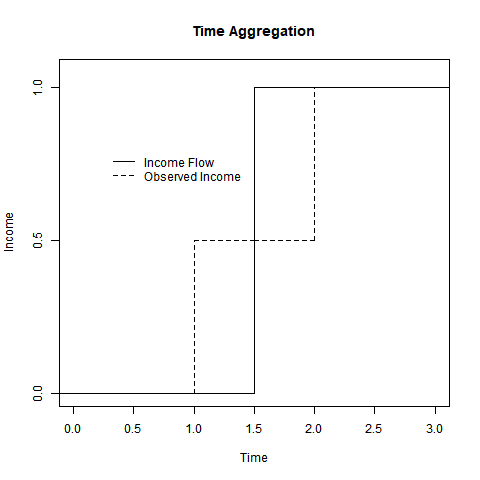
\includegraphics[height=5cm]{../Figures/TimeAggExample2.png}};
	}
	\end{tikzpicture}
	}
	\column{0.5\linewidth}
	\onslide<3->{
	PIH Example:\\
	\begin{itemize}
	\item MPC out of Permanent Shocks = 1\\
	\item MPC out of Transitory Shocks = 0\\
	\item Variances approx. equal
	\end{itemize}
	BPP method estimates MPC out of transitory shocks to be -0.6
	\end{columns}
	}
}
\frame
{
	\frametitle{Aside: Why Not Blundell, Pistaferri and Preston 2008?}
	2) BPP assume consumption is a random walk
	\begin{itemize}
		\item High transitory MPCs are incompatible with consumption following a random walk
	\end{itemize}
}
\frame
{
	\frametitle{Identification of the Income Process}
	We follow the spirit of Carroll \& Samwick (1997):\\
	\begin{itemize}
		\item Permanent income follows a random walk
		\begin{align*}
			p_t = p_{t-1} + \zeta_t
		\end{align*}
		\item Total income includes a transitory component
		\begin{align*}
			y_t = p_t +\varepsilon_t
		\end{align*}
	\end{itemize}
	Growth over N years is:
	\begin{align*}
	\Delta^N y_T &=  (\zeta_{T-N+1} + ... +\zeta_T) + \varepsilon_T - \varepsilon_{T-N} \\
	\mathrm{Var}(\Delta^N y_T) &= N\mathrm{Var}(\zeta) + 2\mathrm{Var}(\varepsilon)
	\end{align*}
}
\frame
{
	\frametitle{Identification of the Income Process}
	We follow the spirit of Carroll \& Samwick (1997):\\
	\begin{itemize}
		\item If transitory income follows an MA(2) process:
		\begin{align*}
			y_t &= p_t + \varepsilon_t + \theta_1 \varepsilon_{t-1} +\theta_2 \varepsilon_{t-2} \\
			\implies \mathrm{Var}(\Delta^N y_T) &= N\underbrace{\mathrm{Var}(\zeta)}_{\text{Perm var}} + 2\underbrace{(1+\theta_1^2+\theta_2^2)\mathrm{Var}(\varepsilon)}_{\text{``Total" trans var}} \text{ if } N\geq 3
		\end{align*}
	\end{itemize}
	Carroll \& Samwick use $N=3,4,5$ to identify permanent shock variance and ``total" transitory shock variance
	\bigskip
	\pause
	\begin{itemize}
		\item[1] How does time aggregation affect this identification?
		\item[2] What might the equivalent of ``robust to MA(2) transitory shocks" be in continuous time?
	\end{itemize}
}
\frame
{
	\frametitle{Identification of the Income Process}
	Carroll \& Samwick in Continuous Time with Aggregation\\
	\begin{itemize}
		\item To begin assume no persistence in the transitory shock
		\item $p_t$ and $q_t$ are independent martingale processes with independent increments
		\begin{align*}
			\mathrm{Var}(p_t-p_{t-1}) &= \sigma^2_p \\
			\mathrm{Var}(q_t-q_{t-1}) &= \sigma^2_q
		\end{align*}
		\item Instantaneous income is equal to the flow of permanent income plus the transitory income component
		\begin{align*}
		dy_t = p_t dt + dq_t
		\end{align*}
	\end{itemize}
	\pause
	We observe $\bar{y}_T$, total income over year $T$:
	\begin{align*}
	\bar{y}_T &= \int_{T-1}^{T}p_t dt + q_T - q_{T-1} \\
	\implies  \mathrm{Var}(\Delta^N \bar{y}_T) &= (N-\frac{1}{3})\sigma_p + 2\sigma_q
	\end{align*}
}
\frame
{
	\frametitle{Identification of the Income Process}
	Allow a generic persistence in transitory shock
	\begin{itemize}
		\item Following shock, transitory income flow decays as:
		\begin{align*}
			f(t)  \text{ where } f(t)=0 \text{ if } t>2
		\end{align*}
	\end{itemize}
	\vspace*{-0.15in}
	\begin{figure}
		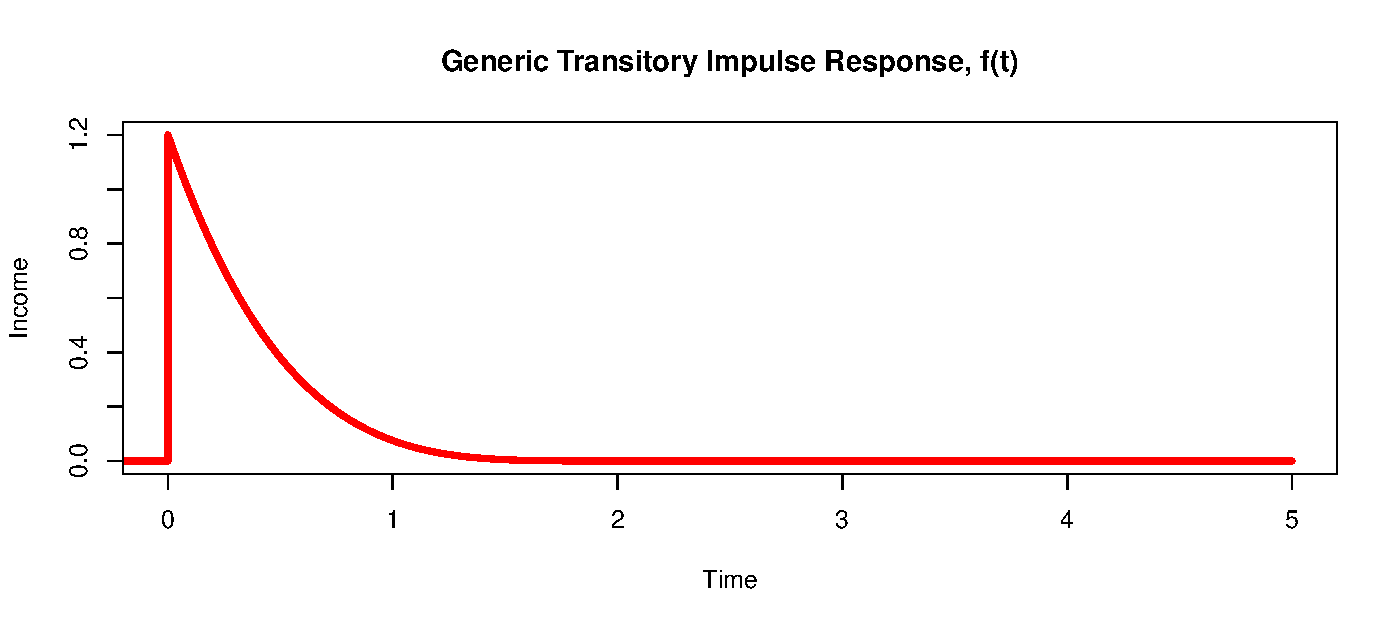
\includegraphics[scale=0.3]{../Figures/GenericTransitory.pdf}
	\end{figure}
	\vspace*{-0.15in}
	\begin{align*}
	y_t &= p_t + \int_{t-2}^{t} f(t-s)dq_s\\
	\implies \mathrm{Var}(\Delta^N \bar{y}_T) &= (N-\frac{1}{3})\sigma^2_p +  2 \sigma^2_{\tilde{q}} \text{   for }N \geq 3
	\end{align*}	
	where $	\tilde{q_T} = \int_{T-1}^{T}\int_{t-2}^{t} f(t-s)dq_s dt$ is the time aggregated transitory component of income
}
\frame
{
	\frametitle{Identification of the Consumption Response}
	Assumptions on Consumption\\
	\begin{itemize}
		\item Permanent: Consumption permanently moves by fraction $\phi$ of the income shock
		\item Transitory: Allow for generic impulse response $g(t)$ where $g(t) = 0$ for $t>2$
	\end{itemize}
	\vspace*{-0.2in}
	\begin{center}
	\begin{tikzpicture}
	\node (img1) {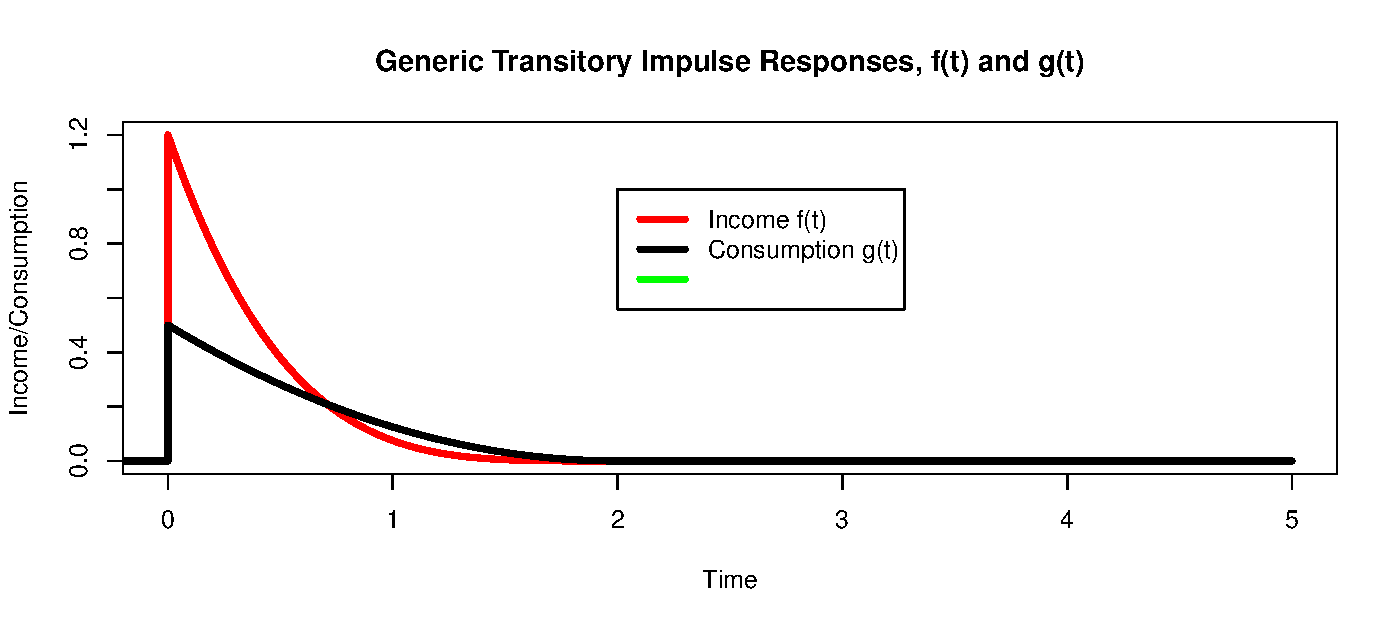
\includegraphics[height=4cm]{../Figures/GenericTransitoryConsumption.pdf}};
	\pause
	\node (img2) at (img1) {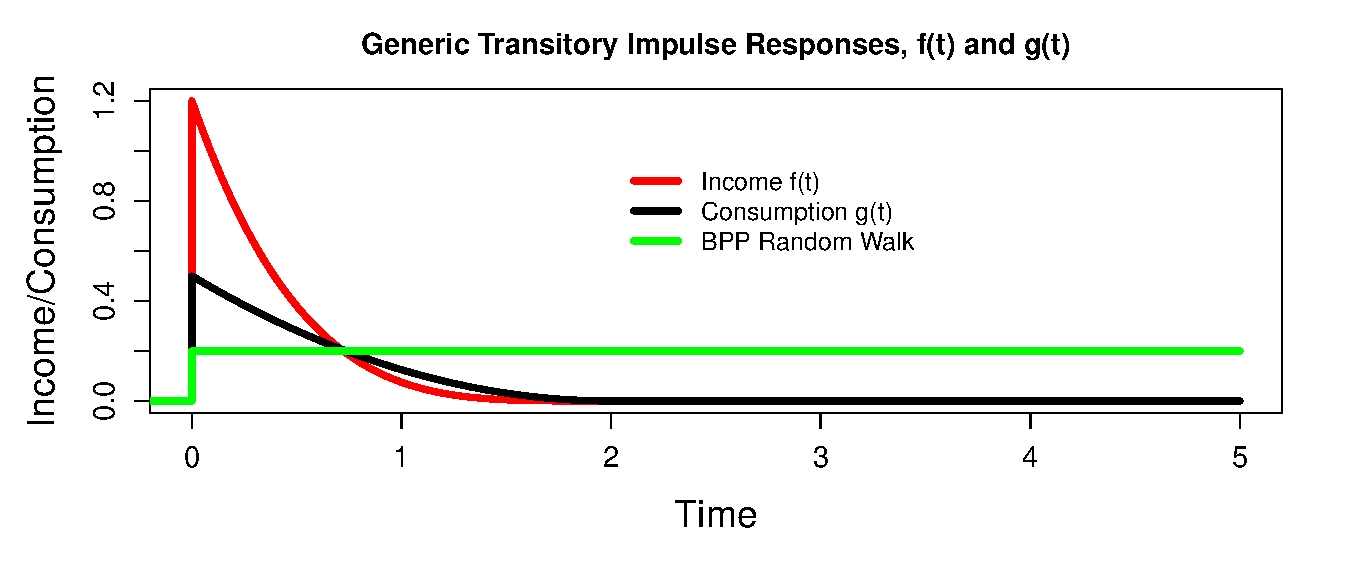
\includegraphics[height=4cm]{../Figures/GenericTransitoryConsumptionWithBPP.pdf}};
	\end{tikzpicture}
	\end{center}
	\vspace*{-0.2in}
	This is a key difference between what we assume and BPP
}
\frame
{
	\frametitle{Identification of the Consumption Response}
	Consumption flow is given by:
	\begin{align*}
	c_t  &= \phi p_t  + \int_{t-2}^{t} g(t-s)dq_s  \\
	\implies \mathrm{Cov}(\Delta^N \bar{c_T},\Delta^n \bar{y_T} ) &= \phi (N-\frac{1}{3}) \sigma^2_p + 2 \psi \sigma^2_{\tilde{q}}
	\end{align*}
	where  $\psi = \frac{\mathrm{Cov}(\tilde{c},\tilde{q})}{\mathrm{Var}(\tilde{q})}$, the regression coefficient of `transitory' consumption on transitory income \\
	\pause
	\bigskip
	\begin{itemize}
		\item $\phi$: MPX out of permanent income shocks
		\item $\psi$: MPX out of transitory income shocks
	\end{itemize}
}
\frame
{
	\frametitle{Full Identification}
We use GMM on the equations:
\begin{align*}
\mathrm{Var}(\Delta^n \bar{y_T} ) &=  (N-\frac{1}{3}) \sigma^2_p + 2  \sigma^2_{\tilde{q}} \\
\mathrm{Cov}(\Delta^N \bar{c_T},\Delta^n \bar{y_T} ) &= \phi (N-\frac{1}{3}) \sigma^2_p + 2 \psi \sigma^2_{\tilde{q}}
\end{align*}
with $N=3,4,5$ (total of six equations) to identify the four unknowns:
\begin{itemize}
	\item $\sigma^2_p$: Permanent shock variance
	\item $\sigma^2_{\tilde{q}}$: (Time aggregated) transitory shock variance
	\item $\phi$: MPX out of permanent income shocks
	\item $\psi$: MPX out of transitory income shocks
\end{itemize}
}
\section{Data}
\frame
{
	\frametitle{Data}
	\begin{itemize}
		\item Starting point: Register based micro data for all Danish households made available by Statistics Denmark
		\item Really good income data
		\begin{itemize}
			\item We use after-tax income for the household head, based on third-party reported tax data
		\end{itemize}
		\item We divide through by permanent income (mean income over all observed years) and take the residual after controlling for age, education, marital status etc. (along with interactions of these)
		\item Expenditure data imputed from income and wealth
		\begin{itemize}
			\item Deposit and brokerage accounts all third party reported
			\item Less accurate than income data
		\end{itemize}
	\end{itemize}
}
\frame
{
	\frametitle{Imputing Expenditure}
	We use the identity
		\begin{align*}
			C_t \equiv Y_t - S_t = Y_t - \Delta NW
		\end{align*}
	\begin{itemize}
		\item Works well for households with simple financial lives
		\item Main issue: Capital gains and losses
		\begin{itemize}
			\item Exclude households where methodology will not work well (eg Business owners)
			\item Exclude housing wealth and years with housing transactions
			\item Capital gains for stocks based on a diversified index
		\end{itemize}
		\item Noisy, but perhaps better than surveys (Browning and Leth-Petersen, 2003; Eika et al., 2017; Fagereng and Halvorsen, 2017; Koijen et al., 2015; Kolsrod et al., 2017; Kreiner et al., 2015)
		\item Huge sample size advantage: sample covers 23.3 million observations over 2004-2015 (approx 1.9 million per year)
	\end{itemize}
}
\section{Results}
\frame
{
	\frametitle{Shock Variance by Age}
	\begin{figure}
		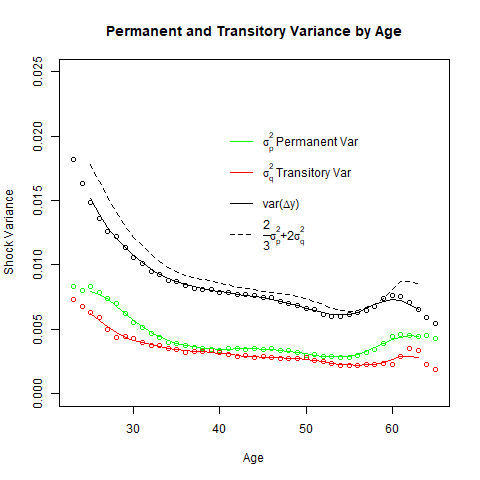
\includegraphics[scale=0.35]{../Figures/VarianceByAge_level_lincome_head.png}
	\end{figure}
	\vspace{-0.25in}
	The assumption of constant variance works reasonably well from mid-30's to retirement
}
\frame
{
	\frametitle{MPX by Age}
	\begin{columns}
		\column{0.5\linewidth}
		\centering
		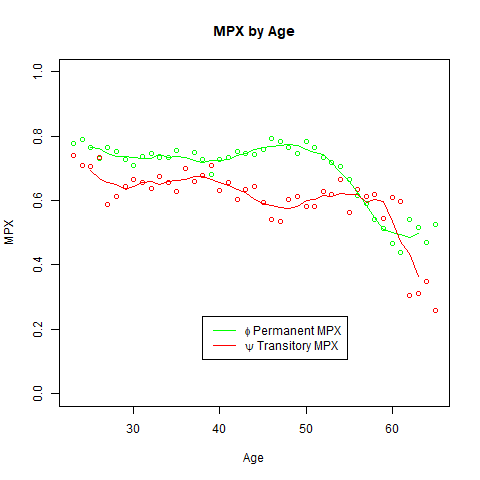
\includegraphics[scale=0.35]{../Figures/MPXByAge_level_lincome_head.png}
		\column{0.5\linewidth}
		\begin{itemize}
			\item $\phi \approx 0.8$, declines towards retirement
			\item $\psi \approx 0.5$, constant
		\end{itemize}
	\end{columns} 	
}
\frame
{
	\frametitle{MPX by Liquid Wealth}
	\begin{columns}
		\column{0.5\linewidth}
		\centering
		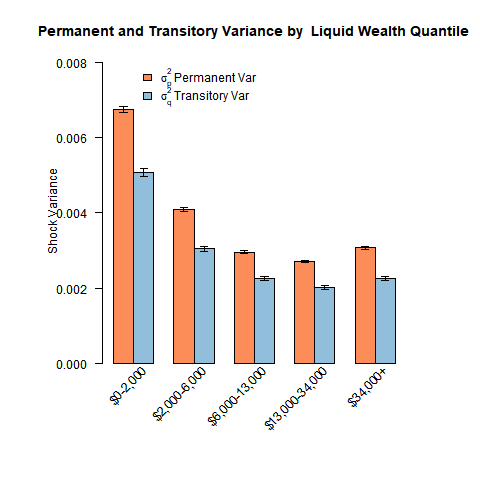
\includegraphics[scale=0.35]{../Figures/VarianceByLiquidWealth_level_lincome_head.png}
		\column{0.5\linewidth}
		\centering
		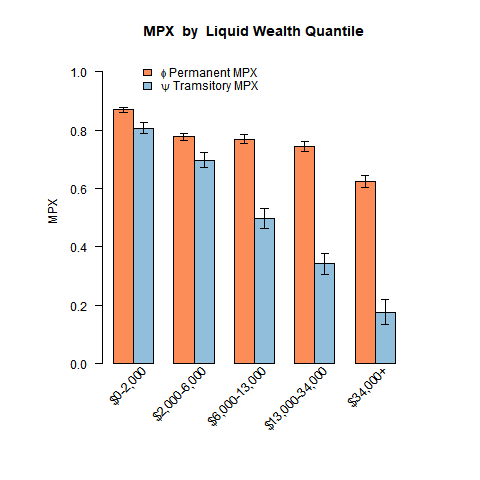
\includegraphics[scale=0.35]{../Figures/MPXByLiquidWealth_level_lincome_head.png}
	\end{columns} 	
}
\frame
{
	\frametitle{Durables}
	Our expenditure measure include ALL expenditure
	\begin{itemize}
		\item Household goods (electronics, kitchen equipment, etc)
		\item Cars
		\item Home improvements (roof repair, extensions)
	\end{itemize}
	Durables make up about 10\% of total expenditure\\
	\pause
	\bigskip
	But theory suggests durable expenditures should not be proportional to permanent income changes 
	\begin{itemize}
		\item This may bias our results
	\end{itemize}
}
\frame
{
	\frametitle{Durables}
	Suppose households \textit{instantaneously} upgrade their durable goods and then pay a constant flow of depreciation:
	\begin{align*}
	dc_t = \phi p_t dt + \color{red} \phi_{d} dp_t \color{black} + \psi dq_t
	\end{align*}
	\begin{itemize}
		\item $\phi$ can be interpreted as the MP\color{red}C \color{black}to permanent shocks, where consumption includes non-durables and the service \textit{flow} from durable goods
		\item $\phi_{d}$ is the proportion of the (annual) permanent shock that is spent instantaneously on durables
		\item $\psi$ is the MPX out of transitory income, exactly as before
	\end{itemize}
	\pause
	Then our estimates of $\phi$ and $\psi$ are unbiased. We have no way of estimating $\phi_d$
}
\frame
{
	\frametitle{Durables}
	If households act with some delay things are different. Suppose they wait 1 year
	\begin{align*}
	dc_t = \phi p_t dt + \color{red} \phi_{d} dp_{t-1} \color{black} + \psi dq_t
	\end{align*}
	\begin{itemize}
		\item $\mathbb{E}(\hat{\phi})=\phi$ Permanent MPC is unbiased
		\item $\mathbb{E}(\hat{\psi})=\psi \color{red} + \frac{\sigma^2_p}{2\sigma^2_q}\phi_d$ Transitory MPX is upward biased
	\end{itemize}
	\begin{figure}
	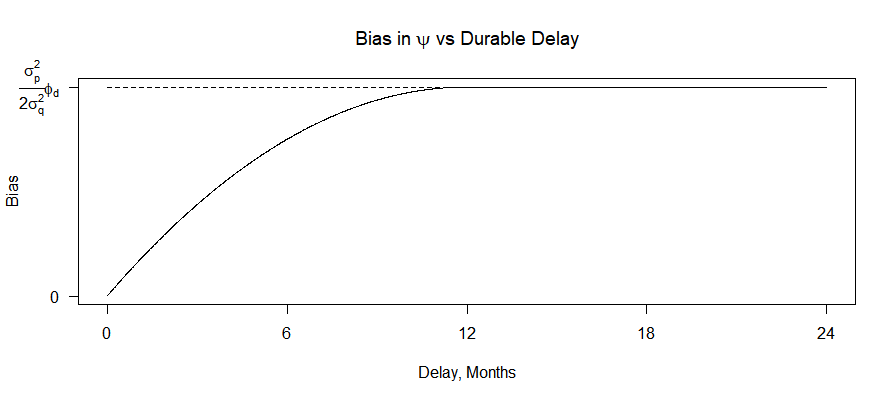
\includegraphics[scale=0.3]{../Figures/DurableBias.png}
	\end{figure}
}
\frame
{
	\frametitle{Durables}
	We have data on value of household cars\\
	\begin{itemize}
		\item Construct expenditure excluding car purchases and sales
		\begin{align*}
		C_T^{\text{nocar}} = C_T - \Delta \text{CarValue}
		\end{align*}
		\item Construct proxy for non durable consumption (Cars $\approx 42.1\%$ durable expenditure)
		\begin{align*}
		C_T^{\text{nondurable}} = C_T - \frac{1}{0.421}\Delta \text{CarValue}
		\end{align*}
	\end{itemize}
}
\frame
{
	\frametitle{Durables}
	\begin{center}
	\begin{tikzpicture}
	\node (img1) {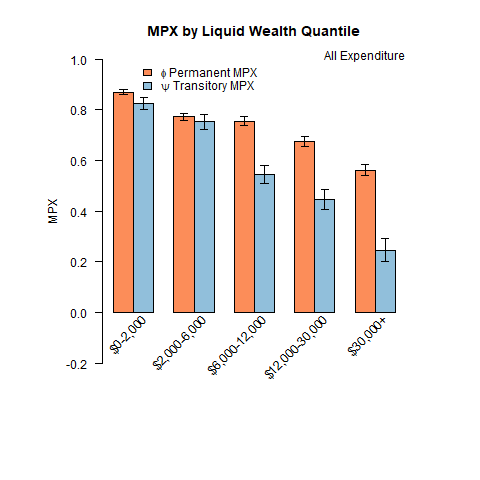
\includegraphics[scale=0.5]{../Figures/MPXByDurables_all.png}};
	\pause
	\node (img2)
	{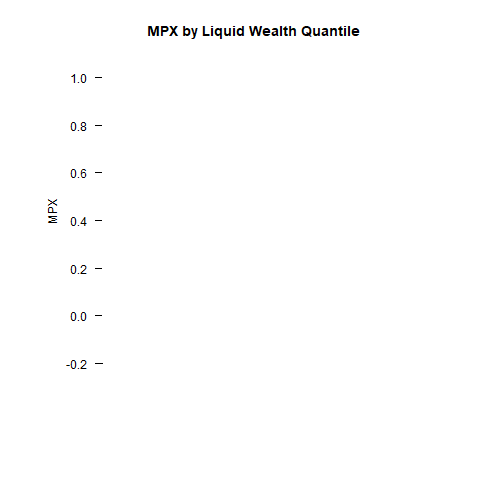
\includegraphics[scale=0.5]{../Figures/MPXByDurables_blank.png}};
	\node (img3) {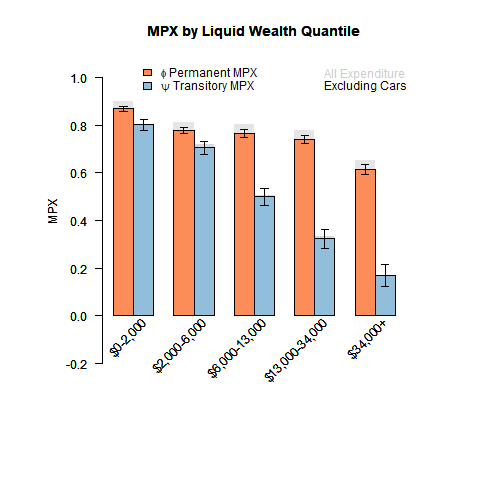
\includegraphics[scale=0.5]{../Figures/MPXByDurables_nocar.png}};
	\pause
	\node (img4)
	{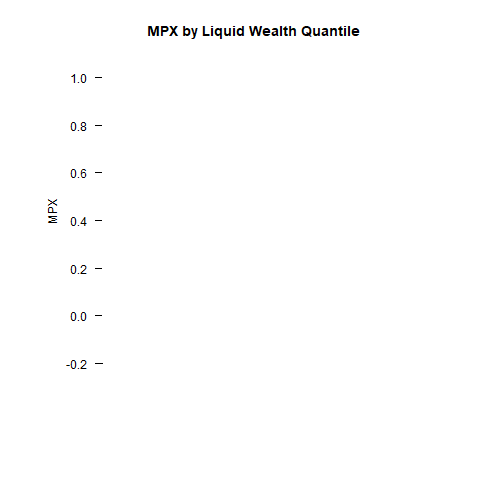
\includegraphics[scale=0.5]{../Figures/MPXByDurables_blank.png}};
	\node (img5) {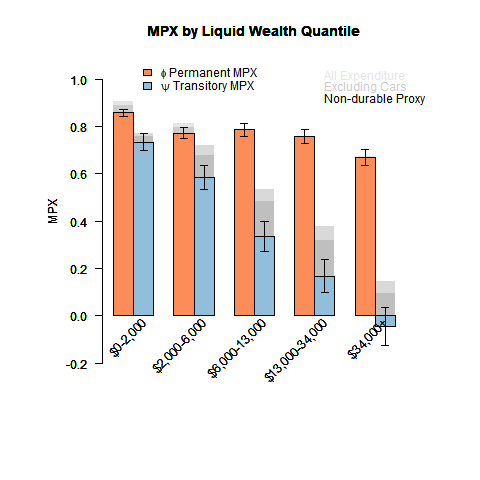
\includegraphics[scale=0.5]{../Figures/MPXByDurables_nodurableproxy.png}};
	\end{tikzpicture}
\end{center}
}
\section{Application}
\frame{
	\frametitle{Monetary Policy: Measuring Redistribution}
	We calculate the sufficient statistics from \cite{auclert_monetary_2015}\\
	\bigskip
	Here we will focus on the \textit{Interest Rate Exposure} channel:\\
	\bigskip
	If\\
	\begin{itemize}
		\item[1] Households that \textit{owe} a lot of floating rate debt have \textit{high} MPCs\\
		\item[2] Households that \textit{own} a lot of floating rate debt have \textit{low} MPCs
	\end{itemize}
	Then lowering interest rates will on average \textit{increase} consumption through redistribution \\
	\pause
	\bigskip
	Do we know if 1 and 2 hold? How can we measure the size of this effect?
}
\frame{
	\frametitle{Monetary Policy: Measuring Redistribution}
	Define \textit{Unhedged Interest Rate Exposure} for household $i$ as the total savings the household will invest at this year's interest rate:
	\begin{align*}
	URE_i = Y_i - C_i + A_i - L_i
	\end{align*}
	Where
	\begin{itemize}
		\item $Y_i = $ Total after tax income 
		\item $C_i = $ Total Expenditure, including interest payments
		\item $A_i = $ Maturing assets
		\item $L_i = $ Maturing liabilities
	\end{itemize}
	Following a change in the interest rate $dR$, the size of the Interest Rate Exposure channell on household $i$'s expenditure is:
	\begin{align}
		dc_i = MPC_i URE_i  \frac{dR}{R}
	\end{align}
}
\frame{
	\frametitle{Monetary Policy: Measuring Redistribution}
	In aggregate, the size of this channel is given by:
	\begin{align*}
	\frac{dC}{C} = \mathbb{E}_I \Big(MPC_i \frac{URE_i}{\mathbb{E}_I (c_i)}   \Big) \frac{dR}{R}
	\end{align*}
	\bigskip
	$\implies$ Need to know the distribution of $MPC_i$ with $URE_i$\\
	\bigskip
	We can do that!
}

\frame{
	\frametitle{Monetary Policy: Measuring Redistribution}
	\begin{figure}
	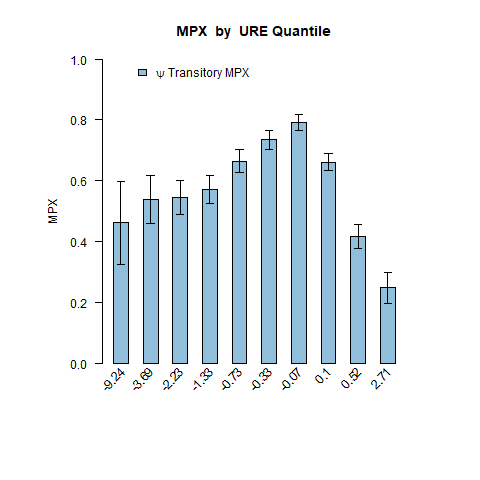
\includegraphics[scale=0.5]{../Figures/MPXByURE_level_lincome_head.png}
	\end{figure}
}
\section{Model}
\frame
{
	\frametitle{Model}
	How does this compare with a standard buffer-stock saving model?
	\begin{itemize}
		\item Build model to match Danish income process
		\item Allow \textit{heterogeneous discount factors} in order to match the distribution of \textit{liquid} assets in Denmark
		\item See how the distribution of transitory MPX varies with liquid asset holdings
	\end{itemize}
}
\frame
{
	\frametitle{Model}
Given market resources ($\boldmath{\mLevBF}_t$), households in this model maximize expected utility:
\begin{align*}
\mathbb{E}_t \sum_{i=t}^{\infty} \beta^i(1-D)^i  u(\cLevBF_i)
\end{align*}
subject to the constraints:
\begin{align*}
\aLevBF_t = \mLevBF_t - \cLevBF_t \\
\bLevBF_t = R\aLevBF_t \\
\yLevBF_t = \theta_t \pLevBF_t \\
\pLevBF_t = \Psi_t \pLevBF_{t-1} \\
\mLevBF_t = \bLevBF_t + \yLevBF_t
\end{align*}
}
\frame
{
	\frametitle{Calibration}
	\input ../Tables/CalibrationTable.tex
}
\frame
{
	\frametitle{Lorenz Curve}
	Lorenz Curve for Liquid Wealth Holdings
	\centering
	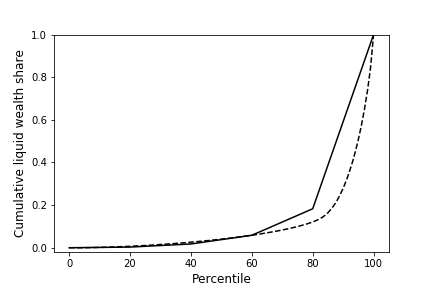
\includegraphics[scale=0.5]{../Figures/Lorenz.png}
}
\frame
{
	\frametitle{Does our Methodology Work?}
	\begin{columns}
	\column{0.5\linewidth}
	\centering
	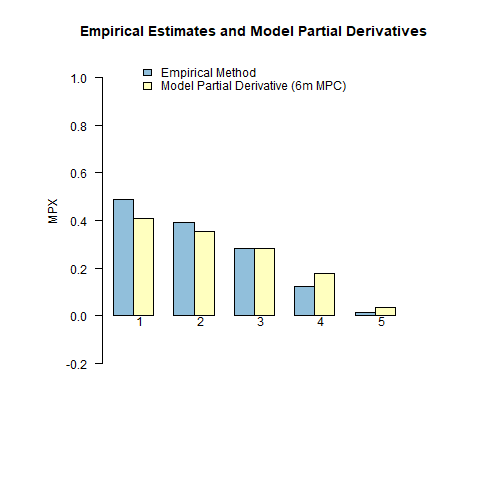
\includegraphics[scale=0.35]{../Figures/MPC_accuracy.png}
	\column{0.5\linewidth}
	\begin{itemize}
		\item Estimate is larger than 6m MPX for low liquid wealth
		\begin{itemize}
		\item Income jumps can be large
		\end{itemize}
		\item Estimate is smaller than 6m MPX for high levels of wealth
		\begin{itemize}
		\item Consumption response lasts more than 2 years
		\end{itemize}
	\end{itemize}
	\end{columns}
}
\frame
{
	\frametitle{Model vs Data}
	How does the model compare with the data?
	\begin{columns}
	\column{0.5\linewidth}
	\centering
	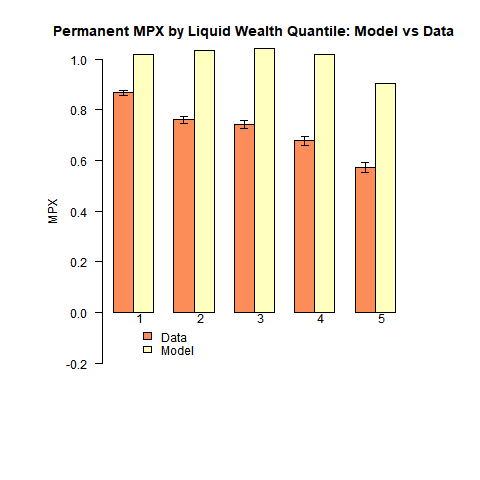
\includegraphics[scale=0.35]{../Figures/CSTW_perm_denmark.png}
	\column{0.5\linewidth}
	\centering
	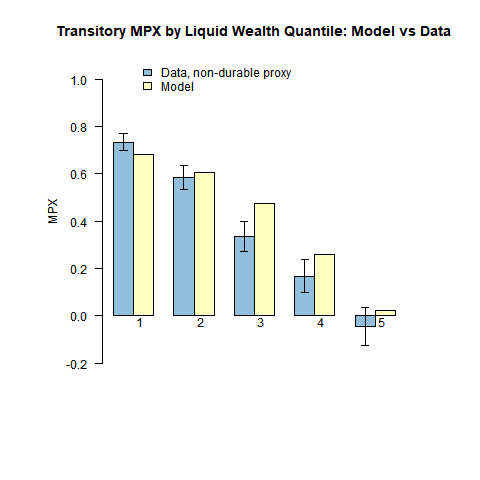
\includegraphics[scale=0.35]{../Figures/CSTW_tran_denmark.png}
	\end{columns} 
}
\section{Threats to Identification}
\frame
{
	\frametitle{Threats to Identification}
  \begin{minipage}{\textwidth}
  \begin{table}
	\label{table:sourcesofbias}
	\begin{tabular}{lcc}  
		\\ & \multicolumn{2}{c}{\textbf{Direction of Bias} }  
		\\ & Perm MPX & Tran MPX
		\\ \hline
		\\ Endogenous Income Shocks & Neutral & +ve
		\\ Persistent Consumption Response & +ve & -ve
		\\ Income Measurement Error &  Neutral & +ve
		\\ Permanent Shocks are AR(1) & Neutral & +ve
		\\ Non-linear MPX	& ? & ?
	\end{tabular}
	\end{table}
	\end{minipage}
}
\frame
{
	\frametitle{Endogenous Income Shocks}
	\begin{itemize}
		\item Household's consumption preference highly variable
		\item Hours worked is endogenous
	\end{itemize}
	The household maximizes:
	\begin{align*}
	\mathbb{E}_t \sum_{n=t}^{\infty} \beta^n \Bigg(\mathcal{X}_n \frac{ \cLevBF_n^{1-\rho}}{1-\rho}-\frac{\lLevBF_n^{1+\frac{1}{\xi}}}{1+\frac{1}{\xi}} \Bigg)
	\end{align*}
	\begin{itemize}
	\item Frisch elasticity $\xi$ 
	\item Preference shock $\mathcal{X}$
	\end{itemize}
}
\frame
{
	\frametitle{Endogenous Income Shocks}
	\input ../Tables/experimental/mpc_laborsupply.tex \\
	\input ../Tables/experimental/psi_laborsupply.tex
}
\frame
{
	\frametitle{Persistent Consumption Response}
	We assume the transitory consumption response lasts less than 2 years \\
	\begin{columns}
	\column{0.5\linewidth}
	\centering 
		High MPC Model\\
	\input ../Tables/experimental/Psi_array1.tex 
	\column{0.5\linewidth}
	\centering
	Low MPC Model\\
	\input ../Tables/experimental/Psi_array2.tex
\end{columns} 
	When MPCs are low, this assumption does not hold in the model, leading to downward bias		
}
\frame
{
	\frametitle{Income Measurement Error}
	Imputation method means measurement error in income shows up in consumption too\\
	Example:
	\begin{itemize}
		\item Actual transitory MPX is zero
		\item 25\% of transitory income variance is due to measurement error
		\item Methodology would result in MPX estimate of 25\%
	\end{itemize}	
	\pause
	But:
	\begin{itemize}
	\item Income is well measured (administrative data)
	\item Bias is much larger for households with small MPCs
	\begin{itemize}
		\item MPX for high liquid wealth households is close to zero
	\end{itemize}
\end{itemize}
}
\frame
{
	\frametitle{Permanent Shocks are AR(1)}
	How does our methodology do if permanent income follows an AR(1) process?
	\begin{align*}
	p_{t} = \rho p_{t-1} + \varepsilon_{t} \\
	y_t = p_t + q_t \\
	c_{t} = \phi y_t + \psi q_t
	\end{align*}
	\centering	
	\input ../Tables/experimental/psi_AR1.tex
}

%%%%%%%%%%%%%%%  bibliography
%%%%%%%%%%%%%%%%%%%%%%%%%%%%%%%%%%%%%%%%%%%%%%%%%%%%%%%%%%%%%%%%%%%%%%%%%%%%%%%%%%%%%%%%%%%%%%%%%%%%%%%%%%%%%%
\tiny

\beamerdefaultoverlayspecification{<*>}
\section{}

\begin{frame}[t,allowframebreaks]
	\frametitle{References}
	
	\bibliographystyle{econtex}
	\bibliography{../AllPapers}
\end{frame}

\normalsize
\end{document}


